\documentclass[twoside]{hcmut-report}
\parindent 0pt
% Draft watermark
% https://github.com/callegar/LaTeX-draftwatermark

\renewcommand{\thesection}{\Roman{section}}
\renewcommand{\thesubsection}{\thesection.\Roman{subsection}}

% Encodings
\usepackage{gensymb,textcomp}

% Better tables
% Wide tables go to https://tex.stackexchange.com/q/332902
\usepackage{array,multicol,multirow,siunitx,tabularx}

% Better enum
\usepackage{enumitem}

% Graphics
\usepackage{caption,float}

% Embed code
\usepackage{listings}
\usepackage{xcolor}
\definecolor{codegreen}{rgb}{0,0.6,0}
\definecolor{codegray}{rgb}{0.5,0.5,0.5}
\definecolor{codepurple}{rgb}{0.58,0,0.82}
\definecolor{backcolour}{rgb}{0.95,0.95,0.92}

\lstdefinestyle{mystyle}{
    backgroundcolor=\color{backcolour},   
    commentstyle=\color{codegreen},
    keywordstyle=\color{magenta},
    numberstyle=\tiny\color{codegray},
    stringstyle=\color{codepurple},
    basicstyle=\ttfamily\footnotesize,
    breakatwhitespace=false,         
    breaklines=true,                 
    captionpos=b,                    
    keepspaces=true,                 
    numbers=left,                    
    numbersep=5pt,                  
    showspaces=false,                
    showstringspaces=false,
    showtabs=false,                  
    tabsize=2
}
\lstset{style=mystyle}


% References
% Use \Cref{} instead of \ref{}
\usepackage[nameinlink]{cleveref}

% Sub-preambles
% https://github.com/MartinScharrer/standalone

% Configurations
\reporttype{Assignment Report}
\title{LINEAR ALGEBRA}
\advisor{Dau The Phiet}
\stuname{%
  & Tran Dinh Dang Khoa    & 2211649 \\
  & Chau Vinh Ky           & 2211785 \\
  & Pham Tan Khoa          & 2252359 \\
  & Pham Tan Phong         & 2252614 \\
  & Nguyen Khac Viet       & 2252904 \\
  & Nguyen Hoang Ngoc Tuan & 2252873 \\
}

% Allow page breaks inside align* environment
%\allowdisplaybreaks{}

% Set depth of numbering for counters (equations, figures, tables, etc.)
% Use package chngcntr if you want more advanced control
\numberwithin{equation}{section}
\numberwithin{figure}{section}
\numberwithin{table}{section}

% Set depth of numbering for sections and table of contents
%\setcounter{secnumdepth}{3}
%\setcounter{tocdepth}{3}

% Custom commands
%\newcommand*\mean[1]{\bar{#1}}

\begin{document}
\coverpage%

\tableofcontents

\clearpage
\section{ Problem 1.}
A code breaker intercepted the encoded message below.\\
45 -35 38 -30 18 -18 35 -30 81 -60 42 -28 75 -55 2 -2 22 -21 15 -10\\[6pt]
Let the inverse of the encoding matrix be $A^{-1} =
\begin{bmatrix}
    w & x \\
    y & z \\
\end{bmatrix}$

\begin{enumerate}[label=(\alph*)]
    \item Given that $[45 \quad -35]A^{-1} = [10\quad 15]$ and $[38\quad -30]A^{-1} = [8\quad 14]$. Write and solve two systems of equations to find $w, x, y,$ and
    $z$.
    \item Decode the message.
\end{enumerate}

\vspace*{1cm}

\textbf{Theory:}\\[6pt]
This problem involves decoding a message that has been encoded using a matrix transformation.\\
To decode the message, we need to multiply each encoded vector by the inverse of A. The inverse of A can be computed using standard methods of matrix inversion, such as Gaussian elimination.\\[6pt]

\textbf{Handwritten solution:}\\[6pt]
We have:
\[
    \begin{bmatrix} 45 & -35 \end{bmatrix}
    \begin{bmatrix} w & x \\y & z \end{bmatrix}
    =
    \begin{bmatrix}
    45w -35y \\
    45x -35z \\
    \end{bmatrix}^T
    =
    \begin{bmatrix} 10 \\ 15 \\ \end{bmatrix}^T
\]

\[
    \begin{bmatrix} 38 & -30 \end{bmatrix}
    \begin{bmatrix} w & x \\y & z \end{bmatrix}
    =
    \begin{bmatrix}
    38w -30y \\
    38x -30z \\
    \end{bmatrix}^T
    =
    \begin{bmatrix} 8 \\ 14 \\ \end{bmatrix}^T
\]

From the above equations, we can write the following system of equations:
\[
\begin{cases}
    45w -35y = 10 \\
    45x -35z = 15 \\
    38w -30y = 8 \\
    38x -30z = 14 \\
\end{cases}
\]

Solve the system of equations using Gaussian Elimination, we get:
\[
\begin{cases}
    w = 1 \\
    x = -2 \\
    y = 1 \\
    z = -3 \\
\end{cases}
\]

Therefore, the inverse of A is:
\[
    A^{-1} =
    \begin{bmatrix}
    1 & -2 \\
    1 & -3 \\
    \end{bmatrix}
\]

After that, we can decode the message by multiplying each encoded vector by the inverse of A.

\vspace*{1cm}

\textbf{Python code:}
\lstinputlisting[language=Python]{code/problem1.py}

\vspace*{0.5cm}

\textbf{Result:}
\begin{figure}[H]
    \centering
    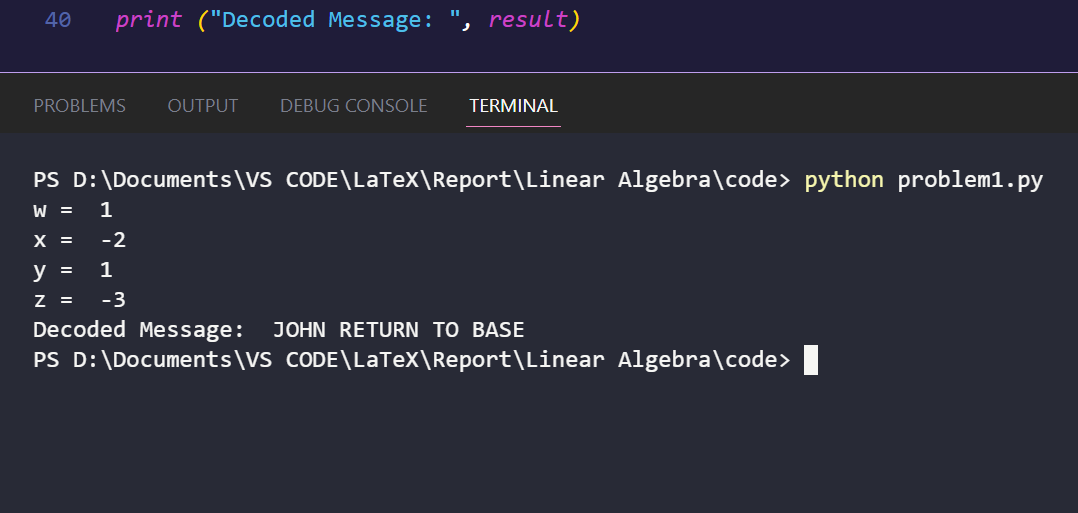
\includegraphics[width=16cm]{graphics/1.png}
    \caption*{Console output of \textit{problem1.py}}
\end{figure}
\clearpage
\section{ Problem 2.}
Construct an inner product in $\mathbb{R}^n$. 
In that inner product, write a program to input any number of vectors in $\mathbb{R}^n$ and return the orthogonal
basis and orthonormal basis of the subspace spanned by these vectors. (Use Gram - Schmidt process). From that, given any vector in $\mathbb{R}^n$, find the coordinates in that basis and find the length of the vector.

\vspace*{1cm}

\textbf{Theory:}\\[6pt]
An inner product in $ \mathbb{R}^n $ is a function that takes two vectors as input and returns a scalar. Mathematically, the inner product of two vectors $ \vec{u} $ and $ \vec{v} $ in $ \mathbb{R}^n $ is defined as:
$$ \langle u, v \rangle = u_1v_1 + u_2v_2 + ... + u_nv_n $$

An orthogonal basis for a vector space is a set of vectors that are mutually orthogonal, meaning that every pair of vectors in the set is orthogonal (their dot product is zero). \\[6pt]
An orthonormal basis for a vector space is a set of vectors that are both orthogonal and normalized. In other words, an orthonormal basis is an orthogonal basis where all vectors have unit length. \\[6pt]
The \textbf{Gram-Schmidt process} is a method for orthonormalizing a set of vectors in an inner product space, most commonly the Euclidean space $\mathbb{R}^n$ equipped with the standard inner product. The Gram-Schmidt process takes a finite, linearly independent set of vectors $S = \{v_1, ..., v_k\}$ for $ k \leq n$ and generates an orthogonal set $S' = \{u_1, ..., u_k\}$ that spans the same $k$-dimensional subspace of $\mathbb{R}^n$ as $S$.\\[6pt]

In order to solve this problem, we need to first prompt the user to enter the dimension of the vector space and the vectors. Then, we need to implement the Gram-Schmidt process to find the orthogonal basis and orthonormal basis of the subspace spanned by the input vectors.\\[6pt]
The simplest and most common inner product for any subspace is the Dot Product. Therefore, we will use the Dot Product as the inner product for this problem.

\clearpage

\textbf{Python code:}
\lstinputlisting[language=Python]{code/problem2.py}

\clearpage

\textbf{Result:}
\begin{figure}[H]
    \centering
    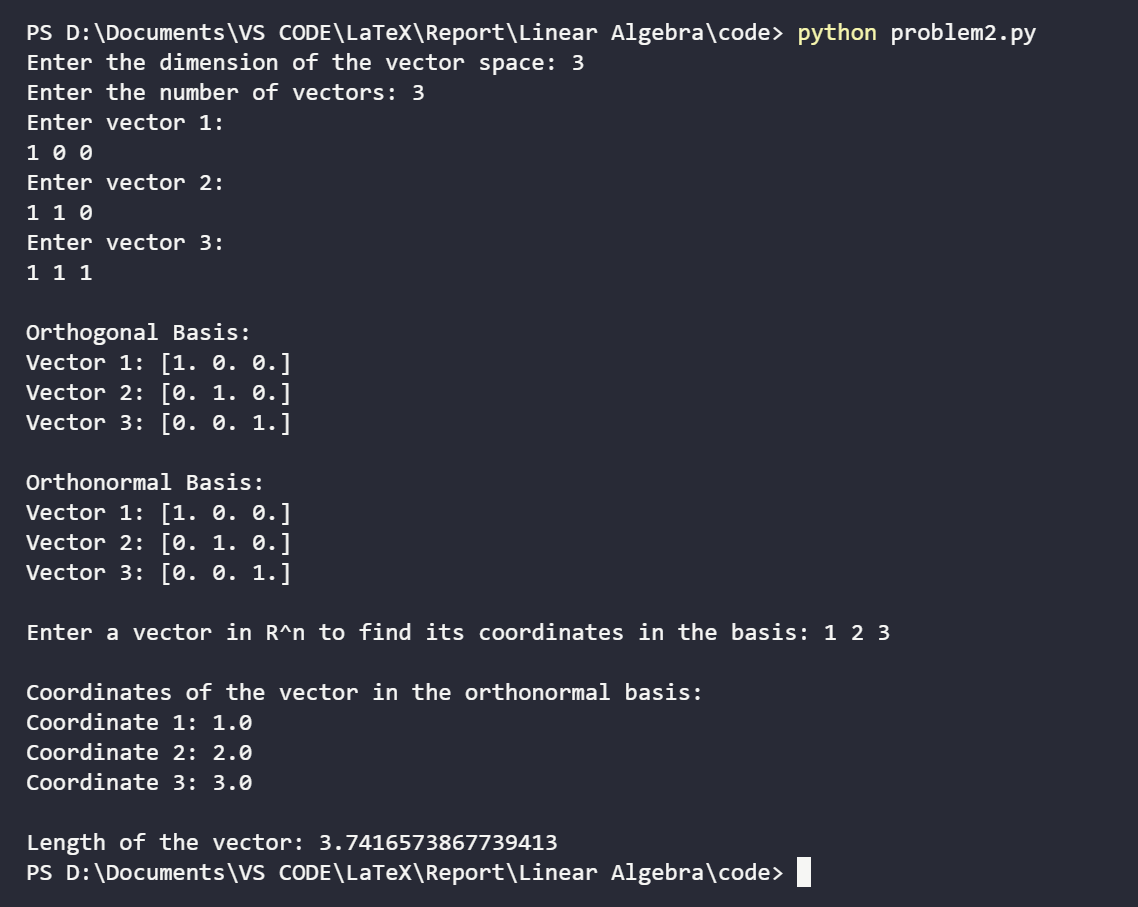
\includegraphics[width=16cm]{graphics/2.png}
    \caption*{Console output of \textit{problem2.py}}
\end{figure}

\clearpage
\section{ Problem 3.}
In $\mathbb{R}^2$, the weighted inner product is given by
$$ \langle x, y \rangle = ax_1y_1 + bx_2y_2 $$
where $a$ and $b$ are positive. Find a weighted inner product such that
the graph represents a unit circle as
\begin{figure}[H]
    \centering
    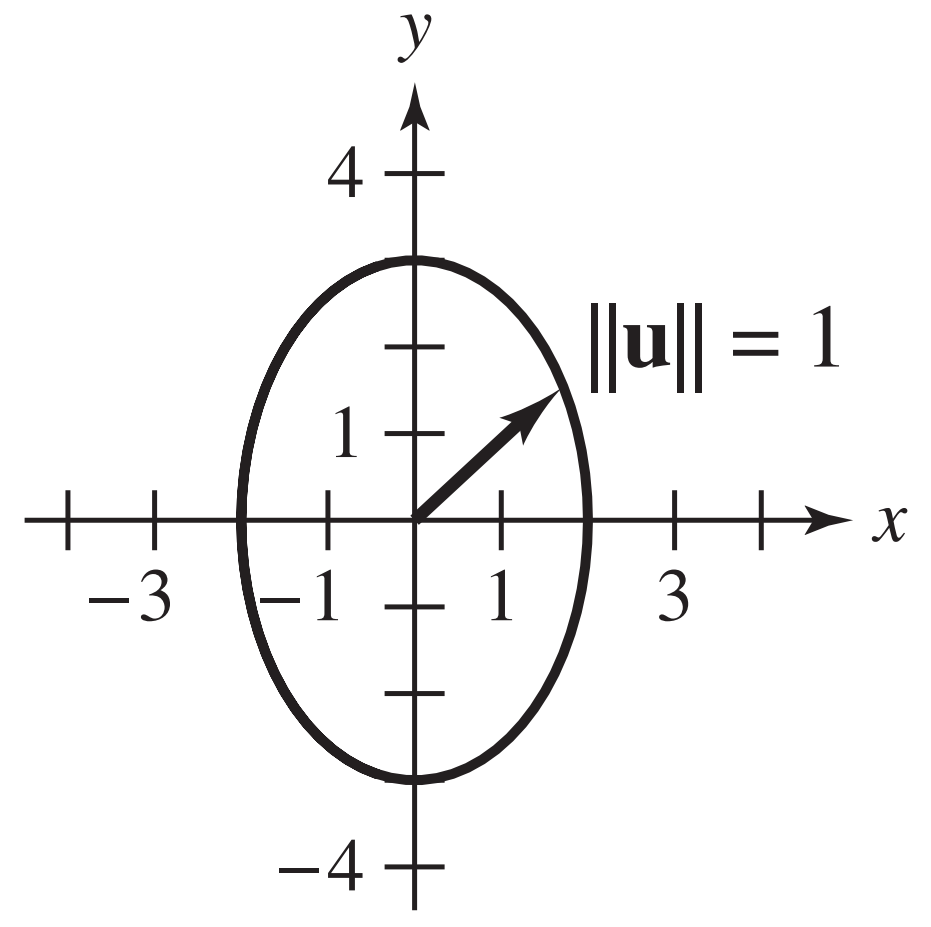
\includegraphics[width=6cm]{graphics/3_0.png}
    % \caption{}
\end{figure}
In that inner product space, reflect that unit circle about an input
plane.

\vspace*{1cm}

\textbf{Theory:}\\[6pt]
Weighted inner products have exactly the same algebraic properties
as the “ordinary” inner product. But they introduce weights or importance factors that modify the calculations and geometric interpretations. \\[6pt]
Let's consider a vector space $V$ over a field $F$. A weighted inner product on $V$ is a function that assigns a scalar value to each pair of vectors in $V$, incorporating weights or importance factors. Formally, a weighted inner product is defined as:
$$ \langle \cdot,\cdot \rangle_w : V \times V \rightarrow F $$
where $\langle \cdot,\cdot \rangle_w$ represents the weighted inner product, and $V \times V$ denotes the Cartesian product of $V$ with itself. \\[6pt]
In a weighted inner product, each component of the vector is multiplied by a corresponding weight or importance factor before the dot product is calculated. This allows for a more flexible and nuanced treatment of vector spaces, where certain components or dimensions may carry more significance or contribute differently to the overall computation. \\[6pt]

In order to solve this problem, we need to first find the weighted inner product such that the graph represents a unit circle. Then, we need to reflect that unit circle about an input plane.\\[6pt]

\vspace*{1cm}

\textbf{Python code:}
\lstinputlisting[language=Python]{code/problem3.py}

\clearpage

\textbf{Result:}
\begin{figure}[H]
    \centering
    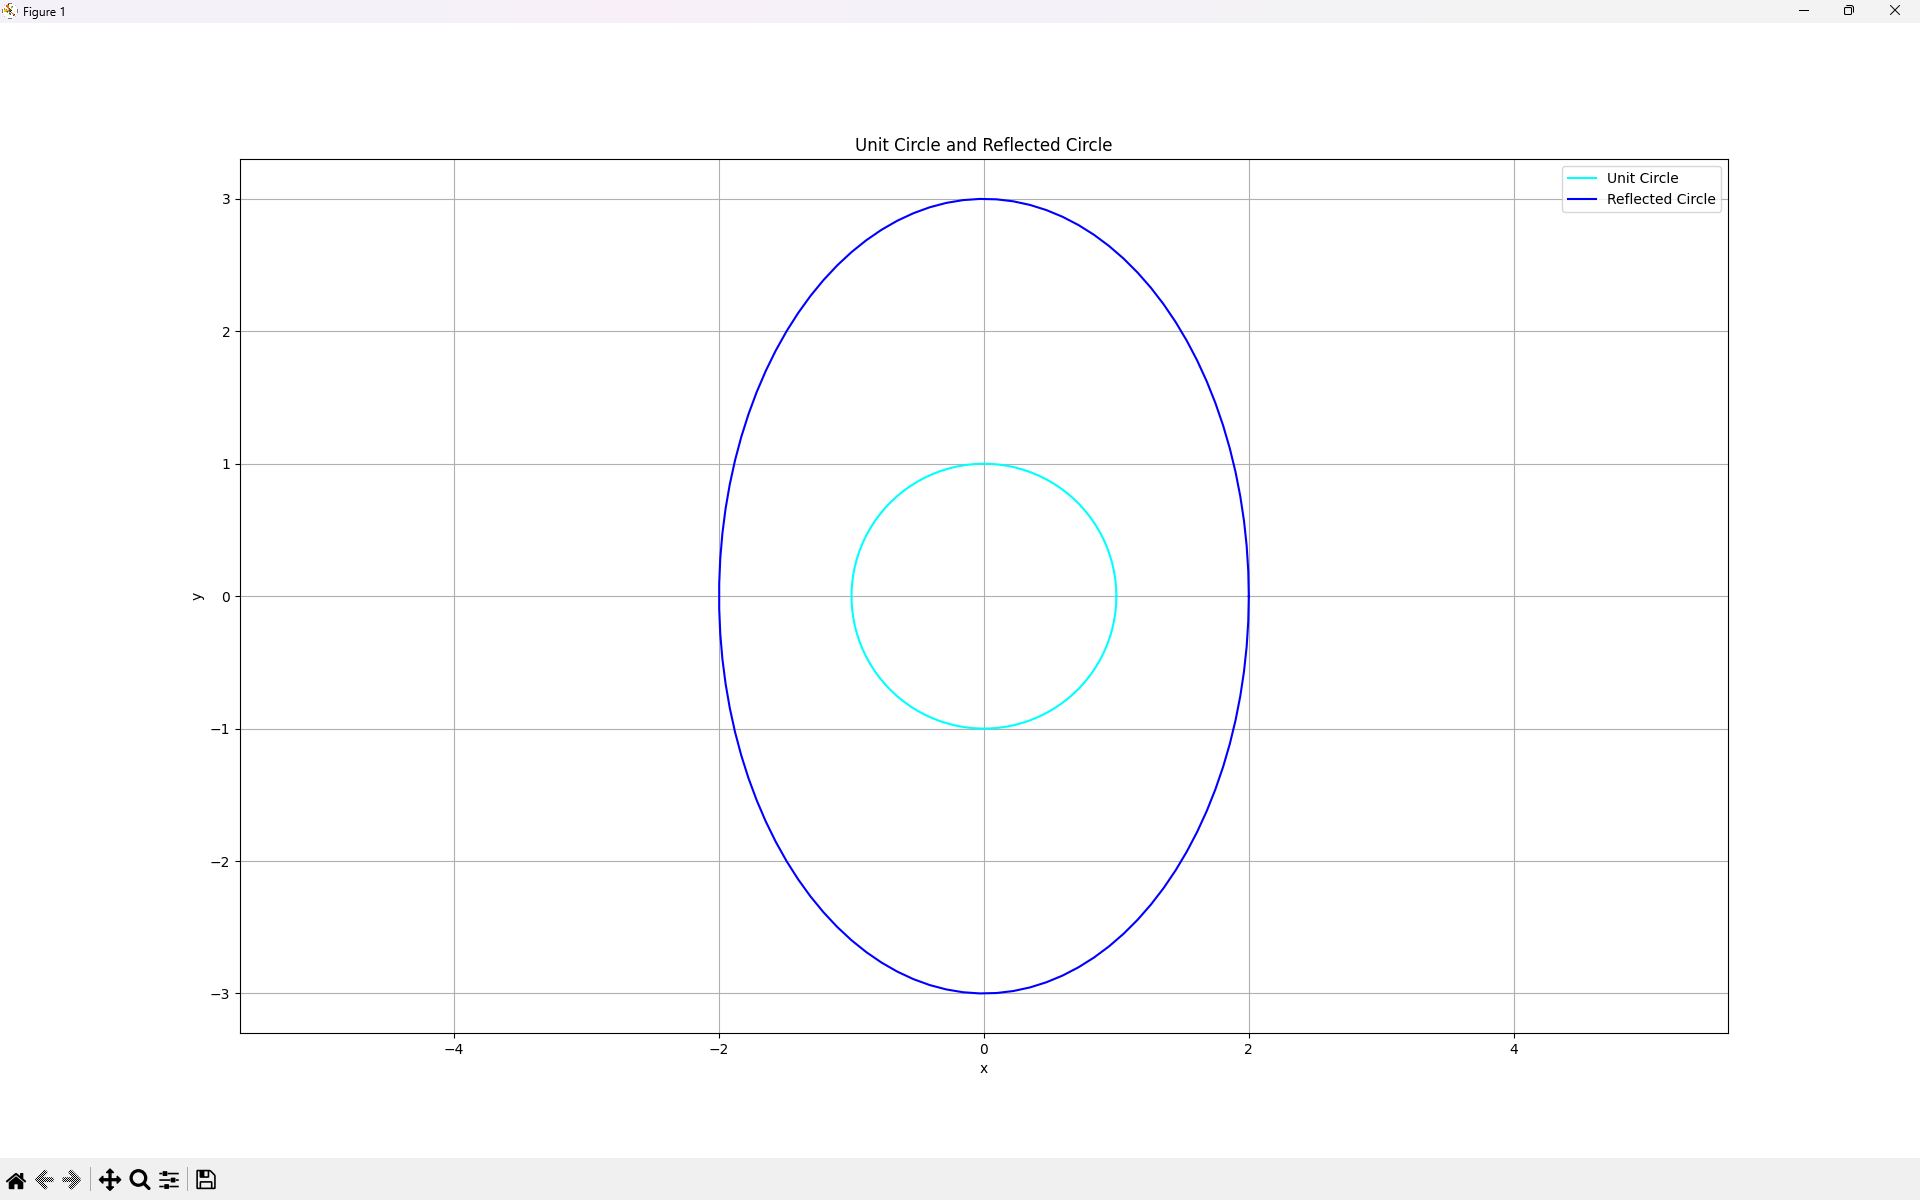
\includegraphics[width=16cm]{graphics/3.png}
    \caption*{Unit Circle and its reflection about the input plane}
\end{figure}
\clearpage
\section{ Conclusion}
This assignment has been instrumental in our exploration of the fundamental principles of Linear Algebra. It has offered us a platform to delve into various key concepts, including matrices, vectors, systems of linear equations, and inner product spaces, all within the context of utilizing Python as a powerful computational tool.\\[6pt]
Throughout the assignment, we have actively engaged with exercises and Python problems, allowing us to solidify our understanding of these foundational concepts. By applying these concepts to real-world scenarios, we have honed our ability to solve practical problems using the tools and techniques of Linear Algebra.\\[6pt]
This assignment has not only expanded our knowledge base but has also contributed to the development of our mathematical skills. By working through the exercises and Python problems, we have sharpened our ability to analyze and interpret mathematical structures and relationships. The hands-on nature of using Python has further strengthened our computational thinking and problem-solving abilities.\\[6pt]
Overall, this assignment has provided us with a valuable opportunity to deepen our understanding of Linear Algebra, develop proficiency in utilizing Python for mathematical computations, and enhance our mathematical skills in a practical context.\\[6pt]

\clearpage
\bibliographystyle{plain}
\bibliography{refs/books.bib}
\nocite{*}

\end{document}
